\chapter{Background}

The topic of this thesis falls into an overlap between the fields of cryptography and machine learning, and as such we will first introduce some concepts from both fields in this chapter.
We will not assume anything more than surface-level knowledge in any of the two fields from the reader.

\section{Cryptography Concepts and \acs{fhe}}

\subsection{Basic Notation and Phrases}

Throughout this work we will use some of the following notations and phrases that are also commonly encountered in other cryptography-related works.
We will introduce these concepts informally aiming for a basic understanding of them while linking to formal definitions.

First we need to introduce the concept of randomness in the context of computational theory.
For this we will use the definitions of \citetitle*{arora_computational_2009} by \citeauthor{arora_computational_2009} \cite{arora_computational_2009}.
Many algorithms in Cryptography rely inherently on randomness and thus cannot be modeled by a standard deterministic \ac{tm} with polynomial programs.
Instead we need to model their computation using the \ac{ptm} which is an extension of the \ac{tm}.
In contrast to the \ac{tm} which only has one transition function $\delta$, the \ac{ptm} has two transition functions $\delta_0$ and $\delta_1$ and chooses at each step at random which one to apply, with probability half to apply $\delta_0$ and half to apply $\delta_1$.

Similarly how $\mathbf{P}$ is the class of decision problems that are solvable in polynomial time by a ac{tm}, $\mathbf{BPP}$ is the class of decision problems that are solvable in polynomial time by a \ac{ptm}.
Note that since the \ac{tm} is a special case of the \ac{ptm} (the one where $\delta_0 = \delta_1$), and since it is possible to simulate all branches of a \ac{ptm} with a \ac{tm} in time $2^{poly(n)}$ it holds that $\mathbf{P} \subseteq \mathbf{BPP} \subseteq \mathbf{EXP}$ (see chapter 7.1 in \cite{arora_computational_2009}).

An alternative definition of a \ac{ptm} would be to add a second tape to a \ac{tm} which includes bits that are results of fair coin tosses, i.e. each symbol on the second tape is chosen mutually independent and uniformly at random from the set $\{ 0, 1 \}$, and then the tape is fed to a \ac{tm} in addition to the regular input tape.
From this viewpoint comes a phrasing of referring to the randomness in cryptographic algorithms like encrypt or key generation functions as 'coins'.
These independent random coin-flips can be viewed as an implicit input to any such algorithm, and are in practice most commonly obtained by pseudo-random number generators.

Furthermore, as introduced in the lecture notes of Mihir Bellare and Phillip Rogaway \cite{bellare_introduction_2005} in chapter 1.3, we will use the following notation to mean that $i$ is a value chosen uniformly at random from the set $\mathcal{S}$: $i \xleftarrow{\$} \mathcal{S}$.
This notation can also be used for algorithms, e.g. $i \xleftarrow{\$} \mathrm{Encrypt}$ which can be viewed as $i$ being a random value from the image of 'Encrypt', or a random result of all possible branches of the \ac{ptm}-equivalent of the 'Encrypt' algorithm chosen uniformly at random.
The \$ denotes the random coins used as input.
Note that some literature may also use $R$ instead of \$.

\subsection{A Simple Somewhat Homomorphic Encryption Scheme: \acs{dghv}}\label{DGHV}

We will begin by introducing a simplified version of an encryption scheme named after \acf{dghv} in \citetitle*{van_dijk_fully_2010} \cite{van_dijk_fully_2010} as an easy to understand example to explain some fundamentals of \ac{fhe} on before moving on to more complicated and current schemes.

This first scheme encrypts bits, so our plaintext space is defined as $m \in \{ 0, 1 \}$.
Our secret key $p$ is an odd integer that is sufficiently large.

We will now encrypt our $m$ into our ciphertext $c$:

\begin{equation}
    c \leftarrow p q + 2 r + m
    \label{eq:dijk_encryption}
\end{equation}

Here $q$ and $r$ are also some integers $\neq p$, sampled at random from some intervals, with $r$ being much smaller than $p$ and $q$.

The ciphertext $c$ can then be decrypted by doing the following:

\begin{equation}
    m \leftarrow \left( c\ \mathrm{mod}\ p \right)\ \mathrm{mod}\ 2
\end{equation}

This encryption scheme is correct because by calculating $\mathrm{mod}\ p$ we get rid of the $p \cdot q$ term in \cref{eq:dijk_encryption} while $\mathrm{mod}\ 2$ nullifies $2r$, with our $m$ staying untouched since it is either 0 or 1 and thus smaller than 2.
Effectively we encode our message in an integer by making it even if it is 0, and odd if it is 1, and then we add $q$ times our secret $p$ to it in order to obfuscate the message.
$p$ is odd, but $q$ can either be odd or even making the result unpredictable.

\begin{remark}
    This is also the reason why $p$ must be odd, if $p$ where even then $pq$ would always be even as well, making the resulting ciphertext even if $m$ is 0, and odd if $m$ is 1, and thus providing no security at all.
\end{remark}

To see why this encryption is secure we first reduce the encryption to the following problem: Given polynomially-many samples (in the security parameter $\lambda$)
\begin{equation}
    \begin{aligned}
        x_1 &= p q_1 + r_1 \\
        x_2 &= p q_2 + r_2 \\
        ...
&\\
        x_n &= p q_n + r_n
    \end{aligned}
\end{equation}
for a randomly chosen odd integer $p$, find $p$.
So in other words the challenger would generate the parameters and then provide the adversary only with $x_1$ to $x_n$, who then would have to find $p$.
Compared to our encryption in \cref{eq:dijk_encryption}, the $x_i$ would be many different ciphertexts, and the $r_i$ would be results of $2r + m$.

While this looks very similar to the well-known \ac{gcd} problem, the key difference here is the random noise $r_i$ which makes the results only approximates of common divisors of $p$.
Because of that this variation is called \acf{agcd}.
While the \ac{gcd} problem can be efficiently solved using Euclid's algorithm, \ac{agcd} with correctly chosen parameters is hard to solve.
While we leave the proof of that to \cite{van_dijk_fully_2010}, intuitively this is the case because when applying Euclid's algorithm the noise values $r_i$ amplify each other rendering the result meaningless.

Finally we will cover the most interesting attribute of this encryption scheme: As long as $r$ stays sufficiently smaller than $p$, multiple ciphertexts obtained from \cref{eq:dijk_encryption} are homomorphic in both addition and multiplication which can easily be shown:

\begin{equation}
    \begin{aligned}
        c_1 + c_2 &= pq_1 + 2 r_1 + m_1 + pq_2 + 2 r_2 + m_2 \\
                  &=p \left( q_1 + q_2 \right) + 2 \left( r_1 + r_2 \right) + m_1 + m_2
    \end{aligned}
    \label{eq:dijk_hom_add}
\end{equation}

Decryption would first remove the first term with the $\mathrm{mod}\ p$ operation, and then remove the second term with the $\mathrm{mod}\ 2$, only leaving $m_1 + m_2$.

\begin{equation}
    \begin{aligned}
        c_1 \cdot c_2 &= \left(pq_1 + 2r_1 + m_1 \right) \left( pq_2 + 2r_2 + m_2 \right) \\
                      &= p^2 q_1 q_2 + 2 r_2 pq_1 + pq_1m_2 + 2r_1pq_2 + 4r_1r_2 + 2r_1m_2 + pq_2m_1 + 2r_1m_1 + m_1m_2\\
                      &= p\left(pq_1q_2 + 2r_2q_2 + q_1m_2 + 2r_1q_2 + q_2m_1\right) + 2\left( 2r_1 r_2 + r_1m_2 + r_1 m_1 \right) + m_1 m_2
    \end{aligned}
    \label{eq:dijk_hom_mult}
\end{equation}

Once again decryption would remove the first term with the $\mathrm{mod}\ p$ operation, and then the second term with the $\mathrm{mod}\ 2$ operation, only leaving $m_1 m_2$.

Please note that because of the $\mathrm{mod}\ 2$ operation, in the case of $m_1 = m_2 = 1$, $m_1 + m_2$ becomes $0$ which is fine since our message space is binary anyway.
So when only looking at the plaintext effectively addition is the XOR-operator and multiplication is the AND-operator.

We can also see some deficits of this simple homomorphic encryption scheme: The noise $r$ grows linearly during addition (see the $r_1 + r_2$ term in \cref{eq:dijk_hom_add}), and quadratically during multiplication ($r_1r_2$ in \cref{eq:dijk_hom_mult}).
Since these homomorphic evaluations only stay correct while the noise is sufficiently smaller than $p$ as already stated, we can only homomorphically evaluate a limited amount of additions and multiplications before decryption would output an incorrect result.
This is why Gentry called these kind of schemes \emph{somewhat} homomorphic encryption schemes in \cite{gentry_fully_2009}, while also providing us with a general algorithm to turn somewhat homomorphic schemes into fully homomorphic ones which we will look at next.

A second deficiency of this scheme is that the ciphertext grows in size during homomorphic evaluation, e.g. after multiplication the 'key-part' of the ciphertext grew quadratically (the $p^2 q_1 q_2$ term in \cref{eq:dijk_hom_mult}).
In other words this scheme doesn't compactly evaluate circuits, as defined by Gentry in definition 2.1.2 and 2.1.3 \cite{gentry_fully_2009}.
Compact Homomorphic Encryption requires the decryption complexity to not by dependent on the circuit depth which in turn requires the ciphertexts and keys (which are the inputs of the decryption algorithm) to not grow with the depth of the circuit.

Finally this scheme in the current form also lacks circuit privacy, another attribute introduced by Gentry in \cite{gentry_fully_2009}.
A regular encryption scheme guarantees that if Bob encrypts a plaintext and sends it to Alice, Alice is not able to infer anything about the contents of the plaintext from the ciphertext.
With homomorphic encryption an additional desired attribute is that, if Alice is performing some operations on Bob's ciphertext, i.e. applying a circuit to it, and then sends the resulting ciphertext back to Bob, that Bob is then not able to infer anything about the nature of Alice's circuit.
He should only be able to decrypt the result of Alice's algorithm, not learn anything about it.
This is called (Statistical) Circuit Private Homomorphic Encryption, since it essentially mandates that the probability distribution of a resulting ciphertext should be the same regardless whether we applied a circuit C homomorphically to it or if we applied the circuit C to the plaintext first and only then encrypted the result.
While our scheme currently doesn't fulfill this attribute, Gentry also points out that most schemes can become circuit private by adding encryptions of '0' to the result many times, randomizing the ciphertext.
Also many schemes only fulfill a relaxed version of circuit privacy where the resulting ciphertext is allowed to reflect the depth of the circuit that got applied to it, but no details of it's exact nature \cite{gentry_fully_2009}.

\begin{remark}
    While we constructed this scheme as a symmetric encryption scheme, in homomorphic encryption any symmetric scheme can be converted into an asymmetric scheme by setting the public key to many encryptions of 0, e.g. in our scheme integers $x_i = q_i p + 2r_i$.
    Anybody can then create a valid ciphertext for their bit m by adding one of the $x_i$s to it.
    For randomization purposes the encrypter should even add multiple $x_i$s to the bit \cite{van_dijk_fully_2010}.
\end{remark}

While this simplified version of the \ac{dghv} scheme is not representative of modern \ac{fhe} schemes, it helps to understand the goals as well as struggles of \ac{fhe} in general.
Most encryption schemes introduce some sort of noise parameter that is strictly required for the security of the scheme, but also introduces limitations regarding accuracy and/or depth of homomorphic evaluation.
Balancing security with these drawbacks as well as handling noise in ciphertexts remain current challenges even with state-of-the-art \ac{fhe} schemes.

\subsection{Bootstrapping}\label{Bootstrapping}

Our previous scheme was only somewhat homomorphic, because it could only evaluate circuits up to a certain depth before the noise got too large for correct decryption.
Because of limitations like this, every homomorphic encryption scheme up until 2009 was not able to evaluate arbitrary computation of arbitrary depth to a ciphertext.
Then Gentry introduced a new quite ingenious technique called \emph{Bootstrapping} in his PhD thesis which enabled him to build the first Fully Homomorphic Encryption scheme \cite{gentry_fully_2009}.

The basic principle behind the bootstrapping approach is to build a somewhat homomorphic encryption scheme that is able to homomorphically evaluate it's own decryption circuit.
It turns out that this decreases the noise of the given ciphertext.
The general strategy becomes to apply computations on the given ciphertext while keeping track of it's noise.
Ones the noise reaches a certain threshold, we apply bootstrapping to get a new equivalent ciphertext with lower noise on which we can then continue our computations until the noise reaches our threshold again and so on.
This means that as long as we can build a somewhat homomorphic encryption scheme that can evaluate computations of the required depth to evaluate it's own decryption circuit plus some additional operations, i.e. if the scheme is bootstrappable, we get a fully homomorphic encryption scheme that can evaluate any circuit on a given ciphertext.

We will now look at bootstrapping in more detail and explain on a high level why it works: We already know that with an homomorphic encryption scheme we can evaluate a function $f$ on some ciphertext $c \xleftarrow{\$} \mathrm{Encrypt}_{sk_1}(m)$ and get the encryption of the result of the function f $\mathrm{Encrypt}_{sk_1}(f(m))$, with $sk_1$ being a secret key.
For bootstrapping, we now introduce a second secret key $sk_2$, and define our function as $f(x) = \mathrm{Decrypt}_x(c)$.
Please note that our function is the decryption algorithm, and that the input of $f$ is not the ciphertext that should be decypted, but the key that should be used to decrypt our ciphertext.
To apply this function homomorphically, we have to provide the input to f, namely the secret key $sk_1$, in an encrypted form, i.e. encrypt the first secret key with a second one.
We will call this encryption of $sk_1$ our bootstrapping key, or $bk$:

\begin{equation}
    bk \xleftarrow{\$} \mathrm{Encrypt}_{sk_2}(sk_1)
\end{equation}

We can now compute our $f$ homomorphically on this bootstrapping key:

\begin{equation}
    \begin{aligned}
        f(bk) \quad (\text{hom. eval. under } sk_2) &\rightarrow \mathrm{Encrypt}_{sk_2}(f(sk_1))\\
                                                    &=\mathrm{Encrypt}_{sk_2}\left( \mathrm{Decrypt}_{sk_1}(c) \right)\\
                                                    &=\mathrm{Encrypt}_{sk_2}(m)
    \end{aligned}
\end{equation}

As you can see, the result is an encryption of the original message under the second secret key $sk_2$.
So by applying the decryption circuit of a ciphertext encrypted under $sk_1$ homomorphically with the encrypted $sk_1$ as input we received a different ciphertext $c_{new}$ that is encrypted under a different secret key $sk_2$.
We effectively switched our ciphertext from one key to another, without decrypting it first or learning anything about the plaintext.
Most importantly, if our $c$ had a high level of noise, the resulting $c_{new}$ has a much lower level of noise enabling further homomorphic evaluation on it \cite{gentry_fully_2009} \cite{dolev_programmable_2021}.

Please note that we used two different secret keys $sk_1$ and $sk_2$ in this explanation which would require switching the ciphertext between encryptions of both secret keys and also requiring two bootstrapping keys $bk_1 \xleftarrow{\$} \mathrm{Encrypt}_{sk_2}(sk_1)$ and $bk_2 \xleftarrow{\$} \mathrm{Encrypt}_{sk_1}(sk_2)$ for repeated executions of the bootstrapping algorithm.
In practice however it is possible to just set $sk_1 = sk_2$ and thus only requiring one bootstrapping key $bk \xleftarrow{\$} \mathrm{Encrypt}_{sk}(sk)$, i.e. the secret key encrypted with itself.
This is called circular security and severely hardens the scheme's security analysis.
Depending on the underlying scheme however it is deemed to be an acceptable practice.

With the bootstrapping algorithm at disposal, constructing an \ac{fhe} scheme became the challenge of building a bootstrappable somewhat homomorphic encryption scheme.
To achieve this Gentry not only tried to increase the maximum circuit depth the encryption scheme could evaluate, but also to decrease the required depth to evaluate the decryption circuit of the scheme.
For \ac{fhe}, the decryption of the underlying encryption scheme must be as computationally efficient as possible, and thus the scheme should also be compact.
Gentry achieved this by not only choosing an encryption scheme that inherently has cheap decryption, but also by squashing the decryption circuit even further at the cost of higher encryption times.
Because of this even modern bootstrappable \ac{fhe} schemes feature very cheap decryption, especially compared to traditional encryption schemes like \acuse{rsa}\ac{rsa} \cite{gentry_fully_2009}.

\subsection{The Path to Modern \acs{fhe} Schemes}

Because of many of the limitations we discussed in \cref{DGHV}, the \ac{dghv} scheme and in general schemes defined just over the integers did not proof to be useful in practice.
Most \ac{fhe} schemes rely on more complex constructions, and their security is based on different mathematical problems.
A timeline featuring the most important of these schemes can be seen in \cref{fig:fhe_timeline}.
Most notably today we have two main branches in the \ac{fhe} world:

The \textbf{"Fast Bootstrapping branch"}, which computes with simple single bit operations and focuses on improving the bootstrapping performance during this.
It can evaluate arbitrary circuits with arbitrary depths, and the party who encrypts the inputs doesn't have to know anything about these circuits at encryption time, making these schemes very flexible \cite{chillotti_tfhe_2021}.

The \textbf{"Leveled schemes branch"}, which implement so called Leveled \ac{fhe}.
This approach can only evaluate circuits on encrypted inputs up to a pre-defined depth d.
This depth can be arbitrary, however it must be known at encryption time \cite{gentry_fully_2009}.
Encrypting for deeper circuits means larger cryptographic parameters and slower evaluation times.
While these limitations make these schemes less flexible, they mostly matter if in a specific application the circuit depth is significantly dependent on the input and thus dynamic or just not known beforehand by the party encrypting the inputs.
For example performing inference on a neural network would be an use case where this does not necessarily matter much, since a forward through the model always goes through a fixed amount of layers and thus operations.
It is important to note that leveled schemes may still allow bootstrapping, they just mostly try to avoid it by setting d statically beforehand.
These schemes are also not defined on bit operations, but on integer and (approximate) floating point operations \cite{chillotti_tfhe_2021}.

\begin{figure}[h]
    \begin{center}
        \includegraphics[width=\textwidth]{../figures/fhe_timeline.png}
    \end{center}
    \caption{A timeline of major \ac{fhe} breakthroughs and encryption schemes, ordered by the different kind of schemes \cite{noauthor_continuing_nodate}}
    \label{fig:fhe_timeline}
\end{figure}

In \cref{DGHV} we built a simple homomorphic encryption scheme based on the \ac{agcd} problem.
Most other schemes however (with the \acuse{ntru}\ac{ntru} branch being a notable exception) are based on some kind of lattice problem.
For example the original \ac{fhe} scheme described by Gentry used ideal lattices, though his construction has since been shown to be insecure \cite{gentry_fully_2009} \cite{smart_final_2022}.
Most other modern schemes are based in some way on the \ac{lwe} problem which we will explain in \cref{LWE}, or its polynomial ring version, the \ac{rlwe} problem \cite{smart_final_2022}.
The first scheme to use \ac{lwe} was the \ac{bgv} scheme in 2011 \cite{brakerski_leveled_2012}.
It's improved version \ac{bfv} \cite{fan_somewhat_2012} which came out shortly after, is also considered to be the first truly practical \ac{fhe} scheme \cite{noauthor_continuing_nodate}.
Because we nowadays also know some possible attacks against \ac{ntru}, \ac{lwe}- and \ac{rlwe}-based schemes are more or less the only secure and practical \ac{fhe} schemes in existence \cite{smart_final_2022}.

Another notable mention is the \ac{gsw} scheme introduced by \citetitle*{gentry_homomorphic_2013} in 2013 \cite{gentry_homomorphic_2013}, since the modern \ac{tfhe} scheme that we will mostly focus on in this thesis originated from it and still incorporates design elements from it, like the \ac{rgsw} ciphertext which is a polynomial ring variation of the \ac{gsw} ciphertext.

\subsection{The \acl{lwe} Problem}\label{LWE}

\ac{lwe} was first introduced by Oded Regev in 2005 \cite{regev_lattices_2005}, and is defined as follows:

Let $n \geq 1$ be an integer (our dimensionality), let p be a prime number, and let $s \in \mathbb{Z}_p^n$ be a secret vector.
Now consider the following set of equations

\begin{equation}
    \begin{aligned}
        \langle s, a_1 \rangle + e_1 &= b_1 &\Mod p\\
        \langle s, a_2 \rangle + e_2 &= b_2 &\Mod p\\
        \langle s, a_3 \rangle + e_3 &= b_3 &\Mod p\\
        \vdots&
    \end{aligned}
\end{equation}

Here the $a_i \in \mathbb{Z}_p^n$ are chosen at random uniformly and independently, $e_i \in \mathbb{Z}_p$ are chosen independently according to some probability distribution $\chi: \mathbb{Z}_p \rightarrow \mathbb{R}^+$, and thus $b_i \in \mathbb{Z}_p$.

Now the \ac{lwe} problem is to obtain $s$ when only the $(a_i, b_i)$ pairs are known.
If all $e_i = 0$, solving this becomes trivial using Gaussian elimination on this set of linear equations.
However with sufficiently large errors $s$ becomes unrecoverable using just Gaussian elimination, making this a hard problem solve.
One strategy would be to apply a maximum likelihood algorithm on a set of $O(n)$ of these equations.
This algorithm would try out different vectors $s'$ and test how many it could solve.
The $s'$ that solves the most equation is equal to $s$.
This however requires testing out many possible $s$ by brute-force, which is why it's runtime is in $2^{O(n)}$.
There are no algorithms that improve this runtime significantly, making this problem NP-hard \cite{regev_lattices_2005}.

The \ac{lwe} problem can be reduced to lattice problems such as the \ac{cvp} which makes \ac{lwe} cryptosystems also lattice-based cryptosystems.
To explain this interpretation of the \ac{lwe} problem we will first define a lattice $L$ with the basis $B$ as the set of all vectors that can be built with this basis using integer coefficients:

\begin{equation}
    L = L(B) = \{ Bc : c \in \mathbb{Z}^k \}, B \in \mathbb{R}^{n \times k}
\end{equation}

The \ac{cvp} problem now is, given a basis for a lattice $B$ and a vector $t \in \mathbb{R}^n$, to find a vector $v \in L(B)$ such that this vector is the closest vector to $t$ in the lattice.
In \cref{fig:lattice_cvp} you can see a graphical representation of this for two dimensions and a trivial basis.

\begin{figure}[h]
    \begin{center}
        \includegraphics[width=0.5\textwidth]{../figures/lattice_cvp.png}
    \end{center}
    \caption{A 2-dimensional space containing the lattice with the base $B = ((0,1),(1,0))$ and a real vector $t$ in orange, with the closest lattice point $v$ to it highlighted in green}
    \label{fig:lattice_cvp}
\end{figure}

While solving this looks quite trivial on the picture, please note that the complexity was $2^{O(n)}$, with $n$ being the dimensionality.
Also this is the trivial basis where the shortest vectors of the lattice are already part of it which makes it a lot easier to solve.
For much higher dimensionality and a more suited base this would indeed become very hard to solve \cite{gentry_fully_2009}.

Our definition of the \ac{lwe} problem shares a lot of similarities with the \ac{cvp} problem: The given vectors $a_i$ of each equation can be viewed as one matrix $A$ that would be the basis of our lattice.
The $b_i$ is the given vector $t$ that contains the error and as such is not part of the lattice, and the problem would become to find the vector $c$ (or $s$), that generates the lattice point closest to this vector.

\subsection{\acl{tfhe}}\label{TFHE}

We will know have a closer look at the \ac{tfhe} scheme because all our experiments in the later chapters will be utilizing \ac{tfhe} in some way.
The paper \citetitle*{chillotti_tfhe_2020} was originally introduced in 2016 by the authors \citeauthor{chillotti_tfhe_2020} (hence this scheme is sometimes also called \acuse{cggi}\ac{cggi}) and describes an improved version of the FHEW scheme, most notably regarding performance and functionality \cite{chillotti_tfhe_2020} \cite{chillotti_tfhe_2021} \cite{noauthor_continuing_nodate}.

On a high level, \ac{tfhe} consists of three different types of ciphertexts, and defines a broad set of operations within and across these three ciphertexts.
We will not explain all these operations exhaustively, but just give a broad overview to give some understanding why mapping arbitrary computations to the most efficient set of \ac{fhe} operations might be challenging.

\subsubsection{\acs{lwe} ciphertexts}

First of we will start with \ac{lwe} ciphertexts: These use the \ac{lwe} problem as explained in \cref{LWE}, and encode the message $m$ from a message space $\mathcal{M}$ in what was before the error of the \ac{lwe} equations.
This guarantees that the message cannot be obtained if only the $b_i$ and $a_i$ are known, because if that where possible one could also easily obtain $s$, the hardness of which is guaranteed by \ac{lwe} and the underlying \ac{cvp} on lattices.

\begin{equation}
    b = \langle s, a \rangle + e + \Delta m \Mod p\label{eq:LWE_encryption}
\end{equation}

In \cref{eq:LWE_encryption} you can see how we encrypt the message $m \in \mathcal{M}$ using \ac{lwe}, with $(a \in \mathbb{Z}_p^n,b \in \mathbb{Z}_p)$ being the ciphertext, $s \in \mathbb{Z}_p^n$ being the secret required for decryption, $\Delta = \frac{p}{|\mathcal{M}|}$ being a scaling factor, and $e$ being a random error with $-\frac{\Delta}{2} < e < \frac{\Delta}{2}$.
Please note that $p$ is not a prime number and thus $\mathbb{Z}_p$ not a field anymore, however in practice this turns out to be fine.
Decryption then becomes just computing the inner product between $a$ and $s$, and subtracting that from $b$:

\begin{equation}
    b - \langle s, a \rangle = \Delta m + e \Mod p \xrightarrow{\mathrm{decode}} m\label{eq:LWE_decryption}
\end{equation}

To see how the last decoding step works and to understand the purpose of $\Delta$, we will look at the following construction:

\begin{figure}[h]
    \begin{center}
        \includegraphics[width=0.45\textwidth]{../figures/lwe_message_encoding.png}
    \end{center}
    \caption{An illustration for how a 2-bit message can be encoded and decoded from a $\mathbb{Z}_{48}$ space}
    \label{fig:lwe_message_encoding}
\end{figure}

\Cref{fig:lwe_message_encoding} illustrates how our $\Delta m + e$ term works for $p = 48$, and $m$ being a 2-bit integer (i.e.
$\mathcal{M} = \{ 0, 1, 2, 3 \}$), resulting in $\Delta = 48 / 4 = 12$.
For example, if we now want to encode the message $m=2$ with a random error of $e = 4$, we would get $12 * 2 + 4 = 28$.
Decoding $28$ would be done by dividing by $\Delta$, and rounding to the next multiple of $\Delta$.
Essentially in the image each possible encoded message without any error ($\Delta m$) is one of the blue lines while the red lines represent the thresholds within which the error can freely move the encoded message without changing it's meaning.
If $|e|$ were to grow to $6$ or larger, then we would not receive our original message during decoding anymore \cite{chillotti_tfhe_2020} \cite{chillotti_tfhe_2021}.

We can easily perform both addition (\cref{eq:LWE_addition}) and multiplication with a constant factor $\gamma \in \mathcal{M}$ (\cref{eq:LWE_multiplication}) directly on \ac{lwe} ciphertexts.

\begin{align}
    \mathrm{Addition:} \quad &(a_1, b_1) + (a_2, b_2) \equiv (a_1 + a_2, b_2 + b_2) &\Mod p \label{eq:LWE_addition}\\
    \mathrm{Constant\ multiplication:} \quad &\gamma (a, b) \equiv (\gamma a, \gamma b) &\Mod p \label{eq:LWE_multiplication}
\end{align}

Why these are equivalent and still correct after decryption can easily be seen in \cref{eq:LWE_addition_proof} and \cref{eq:LWE_multiplication_proof}.

\begin{equation}\label{eq:LWE_addition_proof}
    \begin{aligned}
        b_1 &= \langle s, a_1 \rangle + e_1 + \Delta m_1 &\Mod p\\
        b_2 &=  \langle s, a_2 \rangle + e_2 + \Delta m_2 &\Mod p\\
        a' &= a_1 + a_2 &\Mod p\\
        b' &= b_1 + b_2 &\Mod p\\
        b' &= \langle s, a_1 \rangle + e_1 + \Delta m_1 + \langle s, a_2 \rangle + e_2 + \Delta m_2 &\Mod p\\
           &= \langle s, a_1 + a_2 \rangle + e_1 + e_2 + \Delta (m_1 + m_2) &\Mod p\\
           &= \langle s, a' \rangle + e_1 + e_2 + \Delta (m_1 + m_2) \Mod p\\
        \mathrm{Decrypt:} \quad &b' - \langle s, a' \rangle = e_1 + e_2 + \Delta (m_1 + m_2) \Mod p\\
        (\mathrm{if}\ |e_1 + e_2| < \frac{\Delta}{2}) \quad &\xrightarrow{\mathrm{Decode}} m_1 + m_2
    \end{aligned}
\end{equation}

\begin{equation}\label{eq:LWE_multiplication_proof}
    \begin{aligned}
        b &= \langle s, a \rangle + e + \Delta m &\Mod p\\
        a' &= \gamma a &\Mod p\\
        b' &= \gamma b &\Mod p\\
        b' &= \gamma \left( \langle s, a \rangle + e + \Delta m \right) &\Mod p\\
           &= \langle s, \gamma a \rangle + \gamma e + \Delta \gamma m &\Mod p\\
           &= \langle s, a' \rangle + \gamma e + \Delta \gamma m &\Mod p\\
        \mathrm{Decrypt:} \quad &b' - \langle s, a' \rangle = \gamma e + \Delta \gamma m &\Mod p \\
        (\mathrm{if}\ |\gamma e| < \frac{\Delta}{2}) \quad &\xrightarrow{\mathrm{Decode}} \gamma m
    \end{aligned}
\end{equation}

\subsubsection{\acs{rlwe} ciphertext}

This ciphertext works equivalently to the \ac{lwe} ciphertext, with the only difference being that instead of having integers modulo $p$, we know work with polynomials modulo $X^N + 1$.
The message, secret, our factors, and the error now become polynomials: $M(X), S(X), A(X), B(X), E(X)$, encoding $N$ coefficients.
Encryption and decryption stays equivalent though \cite{chillotti_tfhe_2020} \cite{chillotti_tfhe_2021}:

\begin{align}
    \text{Encrypt: } &B(X) = S(X) \cdot A(X) + E(X) + \Delta M(X) \Mod{X^N + 1}\\
    \text{Ciphertext: } &(A(X),B(X))\\
    \text{Decrypt: } &B(X) - A(X) \cdot S(X) = \Delta M(X) + E(X) \Mod{X^N + 1} \xrightarrow{\mathrm{Decode}} M(X)
\end{align}

Decoding also stays the same, just that the process has to be repeated $N$ times for every coefficient of our polynomial (with $\Delta M_0 + E_0$ for the first coefficient, $\Delta M_1 + E_1$ for the second one, and so on).

On this ciphertext we can also perform addition and multiplication by a constant, except that our constant is a constant polynomial $\Gamma(X)$ this time.
The proofs for why this works are equivalent to the ones we already did for \ac{lwe} ciphertexts \cite{chillotti_tfhe_2020} \cite{chillotti_tfhe_2021}.

\subsubsection{\acs{rgsw} ciphertext}

The \ac{rgsw} ciphertext essentially consists of a multitude of \ac{rlwe} encryptions with additional terms in them, arranged in a 3-dimensional matrix.
Because of it's complex structure we will not explain it in detail and just give a high level overview.
This 3-dim matrix is constructed as $l$ $2\times2$ matrices, where the $j$th $2\times2$ matrix consists of two encryptions of our message: $(A_j(X), B_j(X))$ (the first row), and $(A_j^*(X), B_J^*(X))$ (the second row).
These encryptions differ in the two terms they get in addition to a regular \ac{rlwe} ciphertext \cite{chillotti_tfhe_2020} \cite{chillotti_tfhe_2021}.

\ac{rgsw} allows addition and multiplication with a constant as well which work the same as for \ac{rlwe}, but applied for every single \ac{rlwe} encryption in our matrix.
However additionally it also allows for multiplication between two ciphertexts which was not possible with the last two ciphertexts.

This multiplication works by first decomposing the four polynomials of one of our $2\times2$ matrices from the left-hand site into $l$ smaller polynomials, again returning us a $2 \times 2 \times l$ matrix.
The second step is to perform a matrix multiplication with this decomposition matrix with the right-hand site of our multiplication, returning us a $2\times2$ matrix.
These two steps then have to be repeated $l$ times for every $2\times2$ matrix on the left hand site, combining all $l$ results into one matrix which will then again be a valid \ac{rgsw} ciphertext encrypting $m_1 \cdot m_2$ \cite{chillotti_tfhe_2020} \cite{chillotti_tfhe_2021}.

\subsubsection{Additional \acs{tfhe} building blocks}\label{TFHE_building_blocks}

\ac{tfhe} defines more operations than just addition and multiplication that allow for greater flexibility when implementing arbitrary circuits over ciphertexts, especially when switching between the three different kinds of ciphertexts in \ac{tfhe}.
We give a non-exhaustive list of the most important ones.

The \textbf{External Product} also allows for multiplication between two ciphertexts, with the difference being that on the left-hand side we now have an \ac{rlwe} ciphertext that we multiply with an \ac{rgsw} ciphertext on the right-hand side.
The algorithm works otherwise quite similar to multiplication over two \ac{rgsw} ciphertexts however it works with $1\times2$ matrices instead of $2\times2$ and does not require the $l$ repetitions thus being more efficient.
The result is an \ac{rlwe} ciphertext \cite{chillotti_tfhe_2020} \cite{chillotti_tfhe_2021}.

The \textbf{\ac{cmux}} is a common binary gate with three inputs $d_0, d_1, b$ and one output $d_b$.\label{cmux}
It's function is quite simple:

\begin{equation}
    d_b = \begin{cases}
        d_0 &\mathrm{if\ } b = 0\\
        d_1 &\mathrm{if\ } b = 1
    \end{cases}
\end{equation}

So effectively the \ac{cmux} gate assigns the output to either $d_0$ or $d_1$ depending on $b$.
This is also why \ac{cmux} is so important in \ac{tfhe}, it's being used to implement if-conditions and branching in \ac{tfhe}.
Its implemented using three other operations in the following way (with $\odot$ being the external product, and $-,+$ being addition between \ac{rlwe} ciphertexts):

\begin{equation}
    \mathrm{RLWE}(d_b) = \left( \left( \mathrm{RLWE}(d_0) - \mathrm{RLWE}(d_1) \right) \odot \mathrm{RGSW}(b) \right) + \mathrm{RLWE}(d_0)
\end{equation}

This works because if $b = 1$ this equation will result in $d_1 - d_0 + d_0 = d_1$, but if $b = 0$ then the whole first term will be zero as well and we will be left with just $d_0$ from the second term \cite{chillotti_tfhe_2020} \cite{chillotti_tfhe_2021}.

\textbf{Rotation} allows to rotate the encrypted polynomial of an \ac{rlwe} ciphertext by some $p$ positions, i.e. an coefficient at position $p$ will be at position $0$ after rotation.
This is achieved easily by multiplying the polynomial with $X^{-p}$, and because of the $\mathrm{mod} X^N + 1$ this will automatically rotate the polynomial (plus changing the signs of the coefficients 'falling of' at the left):

\begin{equation}
   \begin{aligned}
       M(X) &= M_0 + M_1 X + ... + M_p X^p + ... + M_{N-1} X^{N-1} &\Mod{X^N + 1}\\
       M(X) \cdot X^{-p} &= M_p + M_{p+1} X + ... + M_{N-1} X^{N-1-p}-M_0X^{N-p} - ... - M_{p-1}X^{N-1} &\Mod{X^N + 1}
   \end{aligned}
\end{equation}

This can be extended to a \textbf{Blind Rotation}, where $p$ is also encrypted (but under \ac{rgsw}).
This is implemented by having $p$ be encrypted bit-by-bit, i.e. we have encryptions of $p_0$, $p_1$,...,$p_k$ where each $p_i$ is one bit of $p$.
Now for each $p_i$ we can perform the regular rotation by $2^i$ positions, and then combine this with a \ac{cmux} with $b = p_i$, $d_0$ being the unrotated $M$, and $d_1$ the rotated one.
That \ac{cmux} will then effectively output $M(X) \cdot X^{-2^i}$ if $p_i = 1$, and just $M(X)$ if $p_i = 0$.
This has to be repeated $k$ times (for every bit of $p$), and all the results have to be summed up afterwards.
Thus we are now able to rotate an unknown polynomial by an unknown amount of positions \cite{chillotti_tfhe_2020} \cite{chillotti_tfhe_2021}.

\textbf{Sample Extraction} allows to simply extract one of the coefficients of an \ac{rlwe} polynomial.
Remember that since every coefficient in \ac{rlwe} is just an \ac{lwe} encryption, this operation returns an \ac{lwe} ciphertext.
This operation is quite trivial and, in contrary to the other non-Bootstrapping operations, adds no noise to the ciphertext.
It can be used to completely convert an \ac{rlwe} ciphertext to an \ac{lwe} ciphertext by simply repeating the process for each of the \ac{rlwe} coefficients \cite{chillotti_tfhe_2020} \cite{chillotti_tfhe_2021}.

\textbf{Key Switching} enables us to change the secret key $s$ under which a ciphertext is encrypted to a new secret key $s'$, without having to decrypt it and without knowing both of the keys.
It requires a so called key-switching-key which can be viewed as a special kind of public-key, and can be performed from \ac{lwe} to \ac{lwe}, \ac{rlwe} to \ac{rlwe}, or even from \ac{lwe} to \ac{rlwe} and many-\ac{lwe} to 1-\ac{rlwe} ciphertexts.
In addition to changing the encryption key it can also be used to change any other cryptographic parameters of the ciphertext, or to even evaluate arbitrary functions on the ciphertext which is called Functional Key Switching \cite{chillotti_tfhe_2020} \cite{chillotti_tfhe_2021}.

We already described the main goal of \textbf{Bootstrapping} (the reduction of noise) and the general function of it in \cref{Bootstrapping}.
In \ac{tfhe} this is implemented on \ac{lwe} ciphertexts, i.e. this algorithm executes the \ac{lwe} decryption (see \cref{eq:LWE_decryption}) homomorphically.
It achiees this quite efficiently using the building blocks described above, more specifically a combination of (blind) rotation, \acp{cmux}, and the Key Switching to move back to the original decryption key.
Since this algorithm is quite complex we will not describe it here in more detail, you can refer to the linked sources for a more in-depth explanation.
Please note that even though the Bootstrapping process uses two different encryption keys, \ac{tfhe} still relies on circular security because of the Key Switching Key which is an encryption of itself \cite{chillotti_tfhe_2020} \cite{chillotti_tfhe_2021}.

\ac{tfhe} also includes multiple more elaborate bootstrapping techniques like \textbf{Gate Bootstrapping}, \textbf{\acf{pbs}}, and \textbf{Circuit Bootstrapping}.
The first two are extensions to the regular \ac{lwe} Bootstrapping that additionally allow the execution of binary gates or any function that can be expressed using a look-up table \cite{chillotti_tfhe_2020} \cite{chillotti_tfhe_2021} \cite{dolev_programmable_2021}.
Using this the bootstrapping becomes more than a pure no-operation that just adds computation overhead since it can now also compute parts of our circuit while decreasing the noise at the same time which increases efficiency.
The third Bootstrapping technique can also execute functions, but most importantly it converts \ac{lwe} into \ac{rgsw} ciphertexts \cite{chillotti_tfhe_2020} \cite{chillotti_tfhe_2021}.

\begin{figure}[h]
    \begin{center}
        \includegraphics[width=\textwidth]{../figures/tfhe_building_blocks.png}
    \end{center}
    \caption{Major \ac{tfhe} building blocks and how they convert between \ac{tfhe} ciphertext types. Dotted lines decrease the noise and solid lines do not. Blocks that take two different kinds of inputs like the External Product/\ac{cmux} or Blind Rotation are represented slightly inaccurately.}
    \label{fig:tfhe_building_blocks}
\end{figure}

A full graphical overview of the above can be seen in \cref{fig:tfhe_building_blocks}.
Compiling an algorithm for \ac{tfhe} ciphertexts becomes the task of combining these building blocks efficiently while keeping track of the noise of the ciphertext and reducing it if necessary.
\ac{tfhe} has some helpful attributes to help with this, for example it allows for constant monitoring of the noise so that the \ac{tfhe} framework in use can dynamically know when it is best to perform the Bootstrapping.
However this abundance of building blocks and their different characteristics make building an optimized \ac{tfhe} circuit a lot more challenging than one might think, and the efficiency and evaluation overhead introduced by \ac{tfhe} compared to regular clear evaluation is quite dependent on the specific application and algorithm and how well it can be or has been optimized for \ac{tfhe}.

\subsection{Some Inherent Limitations of \acs{tfhe}}

We will now briefly look at some inherent limitations that come with the described construction of \ac{tfhe}.
These limitations may also be applicable to other \ac{fhe} schemes however we will focus on \ac{tfhe} here.

\subsubsection{Only over Integers and Booleans - Quantization}\label{quantization}

Our construction of \ac{lwe} and \ac{rlwe} ciphertexts only allow for a discrete message space with relatively small size which prohibits the usage of floating point numbers.
Furthermore even when only using integers, this limits the size of the integer space we can use and thus the integer precision available to us \cite{chillotti_tfhe_2020}.
Even intermediate values in the \ac{fhe} circuit must be integers as well, intermediate values can only be floating point numbers if they are intermediates of a singular \ac{fhe} operations.
For example $(60 * np.sin(x).astype(np.int64)$ can be turned into a single look-up table operation with \ac{pbs}, with $np.sin(x)$ being an allowed floating point intermediate.
However after multiplication with the constant $60$ the result needs to casted into an integer again since that would need be written inside the \ac{pbs} look-up table \cite{noauthor_concrete_2025-1}.

This necessitates a client-side pre-processing procedure of our encrypted inputs before they can be properly used in an \ac{fhe} circuit, called quantization.
Quantization turns floating point numbers and integers into a specific predefined integer range that can be encrypted and homomorphically computed on.
How large that range differs is in \ac{tfhe} heavily dependent on for example the nature and depth of the \ac{fhe} circuit. For example an FHE circuit that includes non-linear operations implemented with \ac{pbs} requires a much higher degree of quantization since the look-up tables used during \ac{pbs} would explode in size if we where to build them for large and high-precision input and output integers.
The size of the integer range is defined by a $p$ which describes the amount of bits we have to represent an integer in this range.
We will call $p$ the bit-width from now on.
First of we need to define a step size $\Delta$ that describes the distance between two adjacent values in our target integer range:
\begin{equation}
    \Delta = \frac{\max(X) - \min(X)}{2^p - 1}
\end{equation}
This means that larger differences between the minimum and maximum of the set of possible values $X$ as well as smaller bit-widths make the necessary step size larger, resulting in a higher loss of accuracy during quantization \cite{frery_privacy-preserving_2023}.
Now the actual quantization can be performed on a new value from our input space $x \in X$:
\begin{equation}
    q(x) = \left\lfloor \frac{x}{\Delta} \right\rceil + z
\end{equation}
Here $z$ is chosen such that $q(\min(X)) = 0$ so that the bit-width is maximally utilized \cite{frery_privacy-preserving_2023}.

Here we can also see how quantization can severely reduce the inputs precision due to the rounding, and thus also reduce the accuracy of the computations coming after.
For larger step sizes this rounding might change the input values quite a bit, making our FHE computations on these rounded values effectively only approximations of the clear equivalent.

\subsubsection{No Support for Control-Flow Statements}\label{no_control-flow}

We have introduced the \ac{cmux} gate in \cref{cmux} that enables conditional assignment of one of two input values to an output.
However while the \ac{cmux} gate may look like an if-statement we want to point out that it can only be used for assignments, i.e. situations where we choose between two already computed values.
It cannot be used to change the control-flow of our \ac{fhe} circuit, i.e. to dynamically change the set of computations applied on the input depending on the encrypted input value.
In fact, \emph{no \acs{fhe} scheme supports control-flow statements that depend on the encrypted input} \cite{frery_privacy-preserving_2023}.

Intuitively, this makes sense since otherwise one could construct an \ac{fhe} program that decrypts the input value through the use of control-flow statements.
For example if the message space is binary, one could build a program that terminates if the encrypted bit is $1$ but stays in an infinite loop if it is $0$.
The adversary could then find out the encrypted bit by just observing the termination behavior of the program.

One result of this is that, if a program introduces branching, in \ac{fhe} we would need to compute every possible branch of the program, and then select the correct execution after the fact using, for example, the \ac{cmux} block to return the output of the correct branch.
Depending on the specific use case this can significantly increase the execution time of our \ac{fhe} circuit, however it should be noted that this can partially be remedied by parallelization since all the possible branches can be computed in parallel \cite{frery_privacy-preserving_2023}.

\section{Machine Learning Concepts and Model Types}

We will now switch over to introduce some concepts of machine learning that we specifically depended on in our later experiments.
Please note however that these will only be basic overviews and not exhaustive explanations.

\subsection{Logistic Regression}\label{LogisticRegression}

Logistic Regression is a generalization of Linear Regression specifically for the binary classification setting (i.e. not for regression, contrary to its name) and in general one of the simplest supervised learning approaches.

Our model parameters are our weights $w$ and a bias $b$, and we get the predicted probability of a label by calculating the inner produc t between our input vector $x$ with the weights, adding the bias, and applying the sigmoid function to the result.
The sigmoid function essentially just maps it's input to the range $[0, 1]$, so that the models output can be interpreted as a probability for the Bernoulli distribution \cite{murphy_machine_2013}:
\begin{align}
    p(y \mid x) &= \mathrm{Ber} \left( y \mid \mathrm{sigm}\left(\langle w, x \rangle + b\right) \right)\\
    \mathrm{sigm}(\eta) &= \frac{1}{1 + e^{- \eta}} = \frac{e^\eta}{e^\eta + 1}\label{eq:sigmoid}\\
    \mathrm{Ber}(y \mid p) &= \begin{cases}
        p &\mathrm{if}\ y = 1 \\
        1 - p &\mathrm{if}\ y = 0
    \end{cases}
\end{align}

This construction solves the binary classification case, however it can be extended to multi-class scenarios by having one weight vector for each class and summing over all classes in the denominator:

\begin{equation}
    p(y = c \mid x) = \frac{e^{w_c x}}{\sum_{c' = 1}^C e^{w_{c'}x}}
\end{equation}

The loss-function that is minimized in training for this model is the log-likelihood function.
Since it is globally convex and derivable twice it can be minimized using a Quasi-Newton method.
Alternatively \ac{sgd} can be applied for Logistic Regression as well which might be faster, especially for large datasets, possibly at the cost of model accuracy.
\ac{sgd} also has the upside of being an online learning algorithm, i.e. the learning scenario where we can update our model weights one sample at a time and not just across large batches of samples \cite{murphy_machine_2013}.

\ac{sgd} can be used with a variety of loss functions, one of which is called Perceptron.
This is a linear loss that for each sample, adds the computed gradient to the model weights if the classification was incorrect, and doesn't change the weights if it was correct.
A slight variation from this is the hinge-loss, that additionally introduces a margin of 1 to the loss to increase the separation of the decision boundary \cite{murphy_machine_2013}.
A good overview with graphs plotting these loss functions can be found in scikit-learn's user guide \cite{noauthor_stochastic_nodate}.
The main takeaway for this thesis is that all these models perform the same operation during inference, namely the argmax of all the inner products between the different class weights and the inputs:

\begin{equation}
    y' = \argmax_c \langle w_c, x \rangle
\end{equation}

For example in scikit-learn, the LogisticRegression, SGDClassifier, and Perceptron classes all perform this step during inference while employing different training techniques.
The Perceptron class is even a wrapper over the SGDClassifier class that just changes the loss function from the hinge-loss to the perceptron-loss and sets the learning rate to be constant \cite{noauthor_api_nodate}.

\subsection{\acl{cart}}\label{CART}

A \acf{cart}, or a decision tree is a type of model that splits the training data recursively into regions that belong to the same label.
This can be represented by a binary tree, where the leafs contain output labels, and each node makes a comparison between one of our features $x_i$ to a threshold $t_i$.
Depending on whether the feature was smaller or larger than the threshold, we will traverse to the left or right child and continue with the next comparison.
The label in the leaf that we will reach by doing this is our models output.
See \cref{fig:decision_tree} for a visual representation of a simple example dataset and a tree fitted to it.

\begin{figure}[h]
    \centering
    \begin{subfigure}[t]{0.45\textwidth}
        \centering
        \includegraphics[width=\textwidth]{../figures/decision_tree_data.png}
        \caption{The partitioned training data with each region colored in it's label ($y_1$ in red, $y_2$ in blue, $y_3$ in green)}
    \end{subfigure}
    \hfill
    \begin{subfigure}[t]{0.45\textwidth}
        \centering
        \includegraphics[width=\textwidth]{../figures/decision_tree.png}
        \caption{One possible decision tree for this data}
    \end{subfigure}

    \caption{A visualization of a decision tree with depth 3, 2-dim features, and three possible output classes}
    \label{fig:decision_tree}
\end{figure}

Fitting such a model perfectly, i.e. finding the optimal partitioning for the training data is shown to be NP-complete, which is why it is common to use greedy algorithms that approximate the best partitioning for training.
One such algorithm is called Boosting, and it applies a weak learner to weighted versions of the training data sequentially, where the weights are higher for samples that the model mispredicted during the last iteration.
In 1998, Leo Breiman called a shallow decision tree combined with the Boosting algorithm the "best off-the-shelf classifier in the world" \cite{murphy_machine_2013}.

\subsection{\acl{fnn}}\label{FNN}

The \acf{fnn}, also called \acf{mlp} is essentially just a series of Perceptron/Logistic Regression models.
The output of each layer is weighted by a weight matrix and passed through an activation function (also called transfer function) before given to the next layer.
This means that a forward pass for each layer consists of a matrix product between the layers weights and the last layers output, and then applying the activation function.
A neural network always consists of one input layer (the values of the feature vector), one output layer (e.g. the probability values of each possible output label), and at least one hidden layer with an activation function.
Most notably these types of neural networks do not form cycles, in contrary to for example a \acf{rnn} \cite{murphy_machine_2013}.
An example can be seen in \cref{fig:NN}.

\begin{figure}
    \begin{center}
        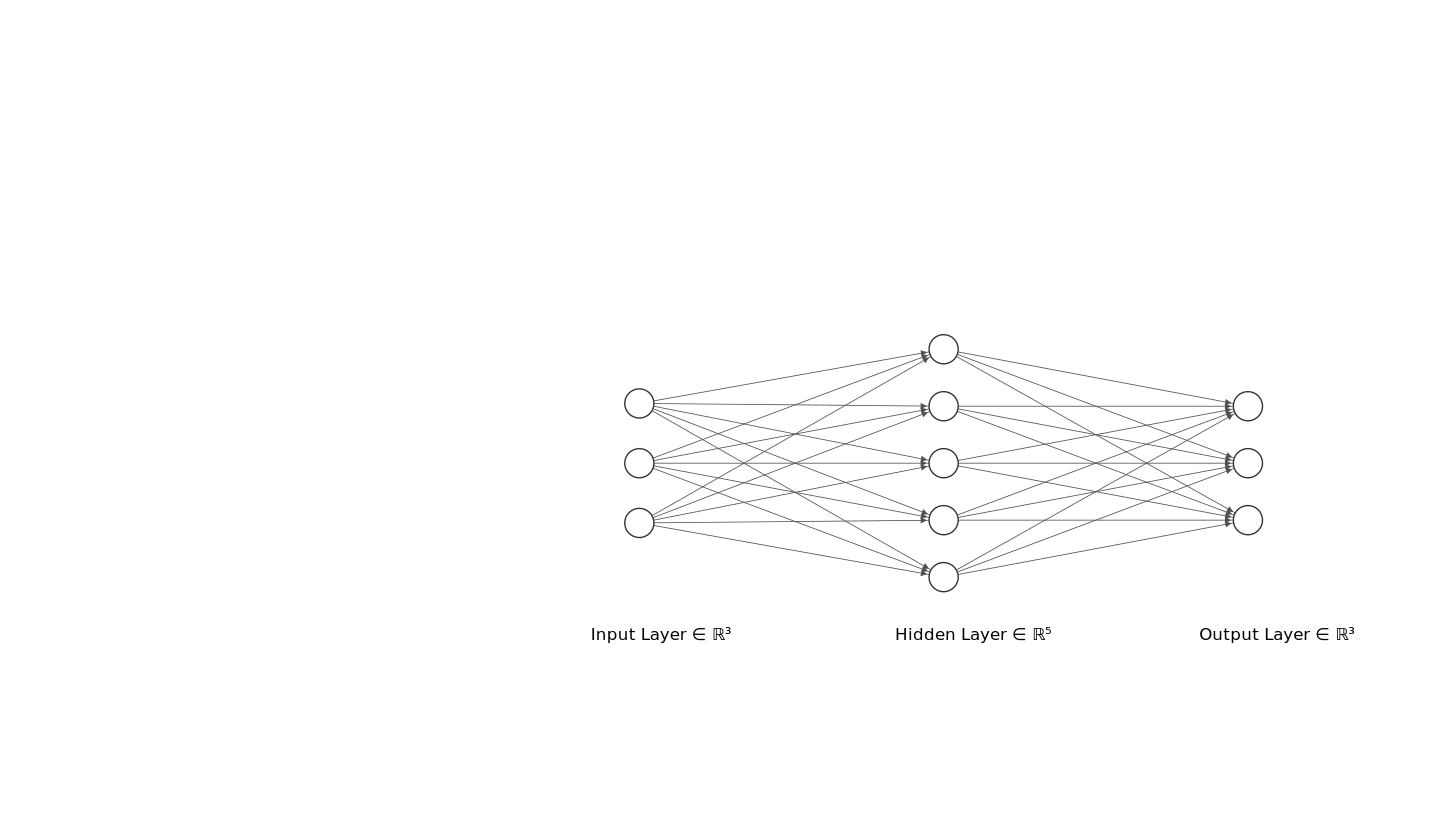
\includegraphics[width=0.95\textwidth]{../figures/nn.png}
    \end{center}
    \caption{A \ac{fnn} with two inputs, two outputs, and one 5-dim hidden layer}\label{fig:NN}
\end{figure}

A model like this (one with only one hidden layer) used for a binary classification problem would thus have the following form:

\begin{equation}
    \begin{aligned}
        z(x) &= g(\langle w_1, x \rangle) \\
        p(y \mid x) &= \mathrm{Ber}(y \mid \mathrm{sigm}( \langle w_2, z(x) \rangle))
    \end{aligned}
\end{equation}

Here $w_1$ are the weights from the input layer to the hidden layer, $w_2$ the weights from the hidden layer to the output layer, $z(x)$ the output of the hidden layer, and $g$ the activation function.
It is important that the activation function is non-linear, since otherwise neural networks would collapse into one large linear model of the form $y = \langle w_1 (\langle w_2 x \rangle) \rangle$.
With suitable non-linear activation functions however it can be shown that this type of model can be a universal approximator that can model any smooth function (given enough hidden units) to any desired level of accuracy \cite{murphy_machine_2013}.

A very common and very simple activation function is the \acf{relu} function, that just cuts any output smaller than $0$:

\begin{equation}
    \mathrm{ReLu}(x) = \max(0, x)
\end{equation}

Other possible activation functions are the logistic sigmoid function (as already defined in \cref{eq:sigmoid}), or the hyperbolic tan function ($\tanh$) \cite{noauthor_api_nodate}.

\subsection{\acl{knn}}\label{KNN}

The \acf{knn} is the last type of model that we will have a look at in this thesis.
In contrary to the previous models it is a non-parametric model.
While parametric models have a fixed set of parameters that are adjusted during training, for non-parametric models such as \ac{knn} the set of parameters grows with the training data.
This is why non-parametric methods are also called memory-based learning, or instance-based learning \cite{murphy_machine_2013}.

Training a \ac{knn} model is quite simple: The model just stores all the feature vector to label mappings that it has seen during training (or a representative set).
For any new feature vector $x$ it will then compute the $K$ geometrically closest training vectors to $x$ according to some metric.
The probability that $x$ belongs to a given label $y = c$ is then the proportion of vectors in $K$ assigned to $c$.
Formally this can be written as follows, where $N_K(x, \mathcal{D})$ are the indices of the $K$ nearest points to $x$ in $\mathcal{D}$:

\begin{equation}
    \begin{aligned}
    p(y = c \mid x, \mathcal{D}, K) &= \frac{1}{K} \sum_{i \in N_K(x, \mathcal{D})} \mathbb{I}(y_i = c) \\
    \mathbb{I}(e) &= \begin{cases}
        1 &\text{if } e \text{ is true}\\
        0 &\text{if } e \text{ is false}
    \end{cases}
    \end{aligned}
\end{equation}

To compute $N_K(x, \mathcal{D})$ most of the time the Euclidean metric is used, however other metrics are also possible and especially useful if our features are not real-valued \cite{murphy_machine_2013}.
A geometric representation of this process can be seen in \cref{fig:knearestneighbors}.

\begin{figure}[h]
    \begin{center}
        \includegraphics[width=0.5\textwidth]{../figures/knearestneighbors.png}
    \end{center}
    \caption{Illustration of two vectors $x_1$ and $x_2$ that are getting classified in a \ac{knn} model by using the training vectors (round points), with $K=3$. $x_1$ has with probability $1$ label $y_1$ while $x_2$ has with probability $2/3$ label $y_2$ and with $1/3$ label $y_1$.}\label{fig:knearestneighbors}
\end{figure}

\ac{knn} can achieve quite good results, and it has even been shown to be able to come within the factor of $2$ to the pest possible classification performance.
However it also has some major downsides: In addition to the growing parameter count which impacts the memory and runtime behaviors of a \ac{knn} model, \ac{knn} notably also suffers from another drawback called the curse of dimensionality.
This effect describes how, with increasing dimensionality of the vectors, we also have to increase the portion of our hyper-space that we consider to be 'neighboring' to our input $x$.
If we want to draw a hyper-cube around our vector $x$ that contains $1\%$ of the data, it's expected edge length has to be $0.01^{\frac{1}{D}}$, with $D$ being our dimensionality.
For $D=3$, we would have to extend the cube to less than $22\%$ in each dimension.
For $D=30$, this would already be almost $86\%$.
The problem with considering such a large proportion of our total space when looking for neighbors is, that the vectors we would compare to our input would not be that similar to it anymore and thus they might not be very good comparison points.
The curse of dimensionality thus results in rapidly declining accuracies of the \ac{knn} model with increasing the dimensionality \cite{murphy_machine_2013}.

\subsection{Some Vectorization Techniques for \acs{nlp} Tasks}

So far we have mostly assumed that our inputs are vectors of numbers (integer or real-valued).
For \ac{nlp} tasks this does not hold true however since our real inputs are text.
There are a lot of preprocessing steps that have to be performed on this text before it can be fed to one of the models we described above.
We will not cover most of these steps, e.g. we will assume that the text has been tokenized already.
We will however look a bit closer at some vectorization techniques, i.e. processes that turn pre-processed tokens (list of strings) into feature vectors (list of integers/floats).
Some of these techniques can be applied to whole documents (i.e. larger excerpts of text), some only for shorter token sequences or just individual tokens.

\subsubsection{One-Hot Encoding and \acl{bow}}

These very simple vectorization techniques generate a vector of dimensionality $|\mathcal{V}|$ for a document and a pre-defined vocabulary $\mathcal{V}$, where each vector entry $x_i$ is one if the word occurred in the document, and zero if not.
For example consider the vocabulary $\mathcal{V} = [ \text{i}, \text{magician}, \text{model}, \text{using}, \text{a}, \text{like}, \text{can} ]$ and the following document:
\begin{verbatim}
    I like using a ML model. I feel like I am using black magic.
\end{verbatim}

With One-Hot Encoding this would get translated into this vector (case insensitive): $[ 1, 0, 1, 1, 1, 1, 0 ]$.
We set the positions corresponding to the vocabulary words that occur in the document to $1$, and the ones that do not occur to $0$ \cite{murphy_machine_2013}.

\acf{bow} is similar except that we do not just encode in the vector whether a vocabulary token occurs in the document or not, but rather how often it occurs.
\ac{bow} would generate the following vector for our example document and vocabulary: $[3, 0, 1, 2, 1, 2, 0]$ \cite{murphy_machine_2013}.

\subsubsection{\acl{tfidf}}

One major problem with \ac{bow} is that we want our features to more uniquely describe their respective documents and their attributes.
Consider for example the use case of sentiment analysis on movie reviews.
This can be implemented as a binary document classification task.
While \ac{bow} would capture all the words contained in each document (that we know from training), most of these words are not relevant at all to the sentiment of the review.
The amount of occurrences of stop words like "a" or "to" for example is very inconclusive for determining the documents sentiment, or most other classification tasks for that matter.

The \acf{tfidf} technique solves this by weighting the frequency of a term inside the document (like we use in \ac{bow}) against the frequency of other documents where this term also occurs.
This means that for our features to become large a token from our vocabulary not only has to occur often in the given document, but it also must occur seldom in other documents.
More formally:

\begin{equation}
    \begin{aligned}
        \mathrm{tf}_{t,d} &= \begin{cases}
            1 + \log_{10} \mathrm{count}(t, d) &\mathrm{if\ } \mathrm{count}(t,d) > 0 \\
            0 &\mathrm{otherwise}
        \end{cases} \\
        \mathrm{idf}_t = \log_{10} \frac{N}{\mathrm{df_t}} \\
        \text{tf-idf}(t,d) = \mathrm{tf}_{t,d} \cdot \mathrm{idf}_t
    \end{aligned}
\end{equation}

Where $t$ is our term, $d$ our document, $N$ the total number of documents, $\mathrm{count}(t, d)$ a function that returns the count of the term $t$ in $d$, and $\mathrm{df}_t$ the amount of documents containing the term $t$ \cite{jurafsky_speech_2025}.

\subsubsection{Semantic Word Embeddings}\label{semantic_embed}

In general a main goal of vectorization is to generate vectors that bring similar data samples close to each other in the resulting vector space, e.g. in classification we would like to have feature vectors to have a high cosine similarity to other vectors of the same output class.
The previous approaches solely relied on frequencies of our terms in the documents which works well for simple document classification tasks.
Other more complex tasks however require our model to gain an intricate understanding of the semantics of any given word and thus it's positional relation to other words in a sentence.

For this we want to generate semantic word embeddings for each word.
These vectors should be similar to one another if and only if they appear in very similar contexts to one another.
For example if two words can be interchanged in most sentences without drastically changing the sentence's meaning or correctness, we would expect the embeddings of these two words to have a very high cosine similarity.
This will not only capture semantic meaning for our model but also automatically deal with synonyms but also homographs (e.g. the "like" in our document example above).

Semantic embeddings are generated by a model specifically trained for this task, like a Word2Vec model or, more commonly nowadays and with much improved results, transformer based models like Bert.
We will not explain the details of these models but refer to a good source instead that covers the topic of textual embeddings more deeply: \cite{jurafsky_speech_2025}.

\subsection{\acl{ner}}\label{ner}

We will now introduce the \ac{nlp} task known as \acf{ner} since we will later use it in our experiments.

\ac{ner} is the task of detecting entity names, e.g. persons, locations, or organisations, in natural text.
Consider the following example:
\begin{verbatim}
    Paris is the capital of France.
\end{verbatim}
Here the tokens 'Paris' and 'France' are named entities, specifically location entities.
At first glance this might look like a simple classification task: Feed the model with the text token-by-token and let it classify each token.
However a model like this would not perform very well in practice since in reality if a token is an entity is highly dependent on the context around the token, not just the token itself.
For example in the following sentence
\begin{verbatim}
    Paris traveled to the capital of France.
\end{verbatim}
the same token 'Paris' now functions as a person's first name. But not just synonyms are problematic:
\begin{verbatim}
    The U.S. Department of the Treasury is the national treasury
    department of the U.S.
\end{verbatim}
Here all tokens of 'U.S. Department of the Treasury' are organisations since it is a multi-token entity, however later on the same tokens 'treasury' or 'department' are no entities at all and 'U.S.' on its own is a location.

A \ac{ml} model that aims to solve this problem well has be able to both consider the context of the token it wants to classify (i.e. the tokens around it), and it needs to learn the semantics of natural languages.
This means it needs to learn the meanings of words and how words restrict the occurrence of words around it.
For example our first two examples are quite similar sentences.
Nonetheless for a human it is no problem to understand that, in the second sentence, the 'Paris' cannot be town.
This is because the verb 'traveled' usually does not apply to locations while the phrase 'is the capital' almost always applies to cities.

There are an uncountable number of rules like these to learn from natural language, making \ac{ner} a quite challenging problem to solve.
